\chapter{Usability}
\section{Usability}
Usability says something about how easy it is to use, learn and understand a human-made system. Examples of systems can be a machines, software applications, websites, tools, or anything else that involves human interaction with an object. Usability is a often used in association with technology development, in terms of making digital systems understandable and intuitive for the users through user-friendly interfaces. Usability has played a huge part in the evolvement of bringing digital systems into people’s homes and everyday life. The first computers and digital systems that were developed consisted of complex and not understandable applications that only professionals with special knowledge could use. There was little focus on simple and accessible systems, and complex interfaces were actually appreciated and gave the system credibility. First, when computers and digital systems were developed with the intention of being used by the normal user, developers had to think about usability. The developers had to put the user in the center of the computer system, and not only focus on functionality and system features \cite{mmi}.

We have experienced a great shift in technology from the first computer was invented and until today. Technology has been more mobile due to laptops, smart phones and other portable devices, and it is also used more often because of instant messaging, e-business and social networks \cite{mmi}. Users are no longer just "computer professionals", but normal people in all age groups, with different skills and interests, that are both experienced and inexperienced with technology. This has been possible because of designers and researchers with focus on human needs. The term human-computer interaction was created, which is about including psychology in developing human-centric design. This is not an easy task, and it includes people from a many different sciences. Ben Shneiderman list “psychologist, instructional and graphic designers, technical writers, experts in human factors or ergonomics, information architects, and adventuresome anthropoplogists and sociologist” as some of the people to be included in the process of saying something about usability and human-computer interaction \cite{mmi}.  

Usability is a wide and quite abstract term, and it is not easy to understand, to measure, or to practise right. ISO 9241 states usability as ".. an important consideration in the design of products because it is concerned with the extent to which users of products are able to work effectively, efficiently and with satisfaction"\cite{usabilitydef}. From this definition we can see that there are three elements that could help us say something about a system's usability; effectiveness, efficiency and satisfaction. Effectiveness measures to which degree the systems covers all necessary functionality, and how easy they are to use and understand. Efficiency is about how well different tasks are performed. This requires measurement on how much time that is used to accomplish a task. The last element is satisfaction, which is about the overall user experience. This could be measures through interviews, studies, questionnaires etc. The degree of satisfaction is important for the system to be accepted \cite{mmi}. 

Making good, intuitive, easy to understand systems is essential for a system to be successful, accepted and used. "Make it or break it" is a slogan that connects well with success and acceptance. A system can possess the best functionality there is, but if the users do not understand how to use it, the system will fail. An example of this is Apple's huge breakthrough when they launched their iPhone in 2007 \cite{iphone2007}. One might associate the invention of the touch phone with Apple's iPhone, but the truth is that touch phones was invented long before the iPhone. The first touch screen was published as early as in 1968, where it was used for air traffic control. In the early 1990s IBM released their Simon, which was the first smart phone with touch screen technology \cite{touchphone}. Apple was also eager participants in the development of touch screen devices. Already in 1983 Apple had a prototype of a touch screen phone \cite{applefirst1983}, and in 1993 they released the world's first Personal Digital Assistant (PDA), called Newton \cite{touchphone}. Apple’s success with their iPhone is based on focus on user’s needs throughout the development process, which has resulted in good, intuitive and user-friendly design and interfaces. "KISS" and "Less is more" is other terms related to usability. "KISS" is an acronym that stands for "Keep it simple, stupid". This term was used in the US navy in the 1960's, and it was a principle stating that simple systems work best than complex ones. The KISS principle has been adopted into the subject of design and usability. Simplicity should be the main focus in design, and every element that leads to unnecessary complexity should be avoided [KILDE - wiki foreløpig]. Ludwig Mies van der Rohe was a German architect that used the term "Less is more" to describe his extreme simplistic and minimalistic design style, and his use of that term became a guiding principle in modern design. "Less is more" has also been widely used as a slogan in association with usability. \cite{rohe}. Minimalistic design can be described as "design at its most basic, stripped of superfluous elements, colors, shapes and textures." With minimalistic design, the most important elements are brought into focus. In this way the user will not be distracted from, or miss out on, the content that is important \cite{lessismore}. Also big companies, like Microsoft, focus on simplicity in their design. Microsoft has launched an article called "The Importance of Simplicity" in their developer network, about how to design user-friendly systems while still keeping good functionality. Microsoft present a topic called "Simple Can Be Powerful". This means that simplistic design not necessarily implies lack of functionality. Simplistic design will provide ease of use for first timers. The idea is to present a design that is intuitive, understandable and easy to learn, but that has the opportunity to build up knowledge about the functionality needed. A possible solution could be to include customisation so the users can set up their own workspace \cite{msdnsimple}.             

There is no definitive solution on how to make a good and user friendly system, and it is challenging and time consuming to find the users needs. For a system design to experience success interaction designers has to pay attention to various aspects of the user. The best way to do this is to involve users in the process of developing the system, from requirement definition and the design phase, to prototype and system test, all to the end of the system's lifecycle \cite{mmi}. When creating something completely new, it is all about understanding what the users want and need, but often the users themselves do not know what they want. It will not be possible to walk up to a potential customer and ask what he or she wants and needs. This does not mean that a developer should be creative, come up with a great idea and bring it into life without ever talking to the user group. The development of a new system should be done as a cyclic process, where development and user involvement goes hand in hand \cite{mmi}.  
\begin{figure} [ht!]
\centering
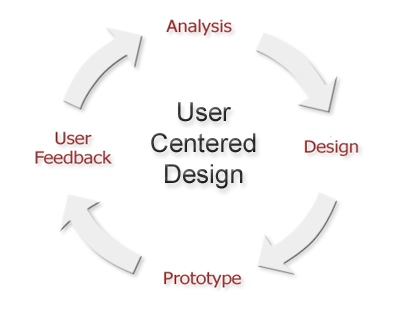
\includegraphics[scale=0.8]{userdesign.jpg}
\caption[User centered design]{User centered design \cite{userdesign}}
\label{userdesign}
\end{figure}

"Participatory design is the direct involvement of people in the collaborative design of the things and technologies they use" \cite{mmi}. Mer brukerinnvolvering fører til mer kunnskap om funksjoner. Gir brukere mulighet til å påvirke hvordan designet ser ut. Innvolvering av brukere i designprossessen kan føre til at de får mer eierskap til produktet, og at det er større sjanse og lavere terskel for at de skal ta det i bruk.

- Gir brukere en stemme i designprosessen, noe som vil øke sannsynligheten for at de vil bruke systemet når det er ferdig 
- Gi en mulighet for utviklere og designere å møte og forså de fremtidige brukerene. 
- Skape et forum for å identifisere og diskutere diverse tema og spørsmål

"We have more to learn than we have to teach", Miller

Hvordan delta. Grupper. Hvordan gjøre det. 

Det å være nøye i utvelgelsen av deltakere kan være med på å lage en positiv og suksessfylt opplevelse. "Competitive selection" øker følelsen deltakerene har av å være viktig, noe som fører til at deltakerene kanskje legger mer i deltakelsen. Det er viktig å fortelle deltakerne hva deres rolle er og hva slags påvirkning de har. De kommer kanskje til å bli spurt om å fungere som en kommunikasjonskanal for en større gruppe som disse deltakerene da representerer. 

http://infodesign.com.au/usabilityresources/participatorydesign/


"Context of use" is an important concept within the definition of usability, and can be defined as "users, tasks and equipment (hardware, software and materials), and the physical and social environment in which a product is used" \cite{maguire2001context}. The degree of quality in user experience for a system is dependent on how well it is related to its specified context of use. A system will be used by a specific population for specific reasons within a specific environment. It is therefore crucial that the system fits the needs of its intended users, functionality, and environment, see Figure \ref{contextofuse}. Analysing a system's context of use will help developers to specify who the users are, what are their characteristics, which functionality do they want, and where and in which circumstances do they want to use it. This understanding about the system can be used all through the development process, from system specification to the test phase \cite{maguire2001context}.

\begin{figure} [ht!]
\centering
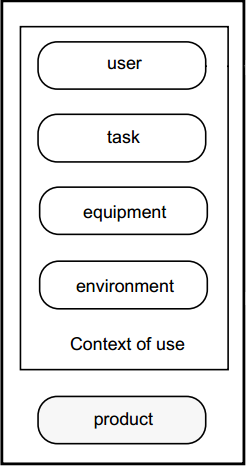
\includegraphics[scale=0.8]{contextOfUse.jpg}
\caption[Context of use]{Context of use, modified from \cite{contextofusefigure}}
\label{contextofuse}
\end{figure}  
  
The work for an interactive system designer is as mentioned to combine the sense of what attracts users with system functionality. To help interface designers make successful systems, a theory called the four pillars of design has been developed. This theory does not guaranteed brilliant systems, but it could be helpful along the way in the development process. The four pillars of design consist of "user-interface requirements", "guidelines documents and processes", "user-interface software tools" and "expert reviews and usability testing" \cite{mmi}.    

\emph{User-interface requirements (Ethnographic observations)}\\
A major key to success when developing a system is connected to specifying the user requirements, and how well these requirements are defined and understood.  The way to specify requirements differs from organisation to organisation, but what the final results should always include the same; Who should use the system, where should it be used and what should it be used for. In addition to this, functional requirements (system requirements like hardware,  software etc.) and non-functional requirements (requirements saying something about the user interface, like functionality, input devices, etc.) should be specified and decided \cite{mmi}.

\emph{Guidelines documents and process (Theories and models)}\\
It is important for the interactive system designer to generate a document that obtains a set of guidelines which specifies how the design should be. Companies like e.g. Apple uses guidelines documents to specify design principles developers should follow. This is to create consistency in design across systems and products. Design may differ as different systems has different needs, but there are still some elements that should be considered in the guidelines document. The documents should contain guidelines for:

\begin{itemize}
\renewcommand{\labelitemi}{$\bullet$}
\item Words, icons, and graphics.
\item Screen-layout issues.
\item Input and output devices.
\item Action sequences.
\item Training.
\end{itemize}

The procedure of creating these guidelines should be done by including different parts of an organisation. It should be a social process, this to gain visibility. It is important that the guidelines are flexible, so that they can adapt to changes in needs and experiences \cite{mmi}. 

\emph{User-interface software tools (Algorithms and prototypes)}\\
In the early stages of development, it is difficult for users to picture what the final result will look like. This may lead to situations where the system design is finished and the users are left with the feeling of not being satisfied. This would be a problem, because of the high cost associated to make changes in implemented systems. One way to address this problem is to let the users get a realistic impression of the final result early in the development process. This could be done by presenting different types of prototypes. These prototypes could be simple sketches on paper, a display proposal or a presentation with use of PowerPoint. When deciding on which development environment to use, there is a number of good products to choose from. Most of them are easy to use, and offers good features. The important part is for the developers to choose the development environment that is most suitable for the product they are going to make, due to performance, cost, and how easy it is to use and learn \cite{mmi}.
	
\emph{Expert reviews and usability testing (Controlled experiments)}\\
To be able to launch a successful system, it is important with testing along the way in the development process. System testing could involve both experts and the intended users \cite{mmi}. 

In order for a system to become successful is has to be easy to interact with. There have been developed a list of eight principles for how to make a good interface design, called "The Eight Golden Rules". This set of guidelines has been developed over three decades with research and experiences. There does not exist a solution for how to make good and user-friendly interface design, but these "Eight Golden Rules" can serve as a starting point and a helpful design guide if they are used correctly. When using the "Eight Golden Rules", it is important that designers refines and implements the principles into the environment they are working in. 

We will now present the "Eight Golden Rules".

\begin{itemize} 
\item \emph{Strive for consistency:} Consistency in interfaces requires identical terminology for actions and layout. This is important for users not to wonder whether words, icons or situations mean the same thing. 
\item \emph{Cater to universal usability:} Designers has to see the need for making a design that fits the diversity of users. There could be differences in age and technology experience, that requires transformation of content. Beginners would need guiding and explanations, while experts should have features for shortcuts. This could improve quality of the system experience. 
\item \emph{Offer informative feedback:} The users should always receive feedback on their actions. Appropriate system feedback should be chosen in accordance to the importance of the actions performed. Process bars, sound as a response for clicking a button, or visual presentation for showing object in actions, is possible ways to give users feedback on actions.  
\item \emph{Design dialogs to yield closure:} It is important to create distinct work steps in dialogs. This means organising similar actions into separate groups with a clear start, middle, and an ending. To provide users with a feeling of accomplishment, feedback should be provided when a particular sequence is finished.     
\item \emph{Prevent errors:} The best solution to this problem would be not to experience any errors at all. Designers should prevent users from doing serious errors by e.g. not allowing inappropriate digits in a field or “hiding” buttons that could cause errors. However, when errors do occur users should be provided with informative instructions for how to recover from the problem.   
\item \emph{Permit easy reversal of actions:} Users should always be provided with the possibility to regret a performed action. This will make the system easy and comforting to use, as users know that every action can be undone. 
\item \emph{Support internal locus of control:} User should feel that they are controlling the interface, and not the other way around. This might be especially important for experienced users. Surprising changes in design and actions, in addition to boring, time-consuming situations, will not be well received. 
\item \emph{Reduce short-term memory load:} Designers should reduce the need for memorising information and how actions should be performed. The focus should be on designing an interface with visible information and intuitive actions.
\end{itemize}

These "Eight Golden Rules" is far from being the only guide for how to design a user interface. There have been done a huge amount of research in the area of usability, where Jacob Nielsen is one of the participants \cite{nielsen2005ten}. Nielsen is a Ph.D from Denmark, and an expert in human-computer interaction. He has established a movement for how to easy improve user interfaces, invented several methods for how to achieve good usability, and he has also published a great amount of articles and books with usability as main subject \cite{JNielsen}. As a part of his work Nielsen has created a list of ten usability heuristics, which can be used as general principles when designing a user interface\cite{nielsen2005ten}. 

\section{Heuristics}
It is clear from this chapter that it is critical to involve the user in the testing of technology systems, to be able to evaluate the playability and the user friendliness. This is because it is impossible for the designer to fully understand or predict the users actual behaviour with a game.  Heuristics are designed guidelines made to assess how good software design is, and it has become a widely used method for usability evaluation in software development. It is important to develop software interfaces that are easy to understand, learn and conduct. With the use of heuristic, this can easily be evaluated. Heuristic evaluation method allows for insight into users' point of view, even before there is an actual system, and is actually best suited in an early phase, before spending a lot of money on expensive prototypes. When prototypes are made, the user needs to be involved to discover problems if they appear. This is also a very important part of the development, because it is critical to understand the interaction between the player and the game \cite{desurvire}. 

A lot of research have been done when it comes to how usability can be tested in the best way. There has been suggested different sets of heuristics in \cite{nielsen2005ten}, \cite{malone}, \cite{shelley}, \cite{federoff}. Many of these overlap, and in some way, they all tell the same.  Desurvire et al. presents a thorough set of heuristics that covers four game heuristic categories:  \emph{Game play}, which is the challenges that needs to be overcome to win the game, \emph{Game Story}, which intuitively is the story of the game and its characters, \emph{Game Mechanics}, which covers the interaction between objects and the game environment, and  \emph{Game Usability}, which is the elements used to be able to interact with the game, like for example a controller. They present a set of heuristics that is based on the already existing literature. The heuristics have also been reviewed by different playability experts and game designers. The model presented by Desurvire et al. proved to be very useful in an early development phase \cite{desurvire}.

Melissa Federoff evaluates in her thesis different sets of heuristics from the literature. With these in mind, she did a case study where she observed and interviewed different members of a game development team. Based on this she removed some heuristics, added some heuristics, and  suggested a new set of heuristics. The list of heuristics that she created in her study can serve as a starting point for the development of a standard list that the game community can use  \cite{federoff}. 

Even though Federoff's study was aimed towards game development, Sweetser and Wyeth discovered that many of the heuristics proposed in the literature, did not evaluated the enjoyment in games. They argue that the many valid sets of heuristics presented in the literature should be integrated in a model where also player enjoyment can be assessed. They suggest a model, which they call "GameFlow". They describe flow as "..based on the premise that the elements of enjoyment are universal and provides a general model that summarises the concepts that are common to everyone when the experience enjoyment (e.g. ability to concentrate on the task)". They argued that the nature of flow fits well as a way to structure the different heuristics found in the literature, into a model of player enjoyment. The "GameFlow" model has eight core elements: \emph{concentration, challenge, skills, control, clear goals, feedback, immersion} and \emph{social interaction}, see Figure \ref{fig:gameflow1} and \ref{fig:gameflow2} \cite{sweetser}. 

\begin{figure} [ht!]
\centering
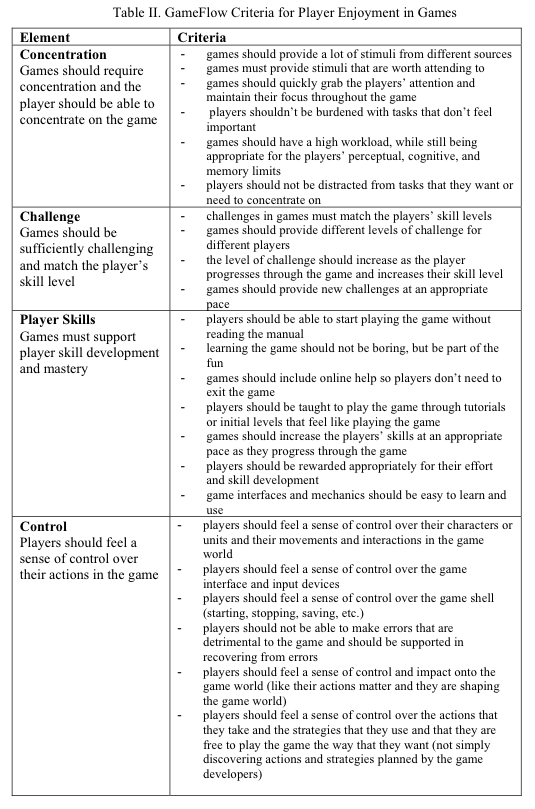
\includegraphics[scale=0.7]{gameflow1}
\caption[GameFlow criteria for player enjoyment in games, part 1]{GameFlow criteria for player enjoyment in games, part 1 \cite{sweetser}}
\label{fig:gameflow1}
\end{figure}  

\begin{figure} [ht!]
\centering
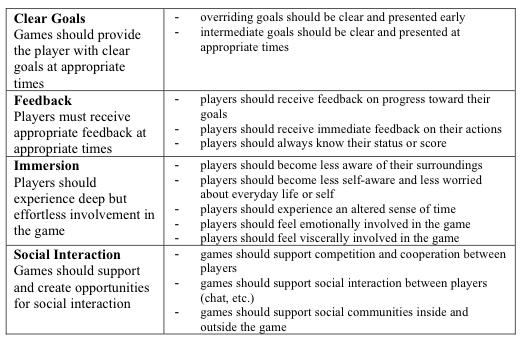
\includegraphics[scale=0.7]{gameflow2}
\caption[GameFlow criteria for player enjoyment in games, part 2]{GameFlow criteria for player enjoyment in games, part 2 \cite{sweetser}}
\label{fig:gameflow2}
\end{figure}  

We will now discuss the eight core elements briefly. We will not discuss every criteria, as they are all presented in Figure \ref{fig:gameflow1} and \ref{fig:gameflow2}, but we will emphasis some of the elements we find important. 

For the game to be fun, the player needs to be able to concentrate on the tasks. The players attention and concentration should be maintained throughout the whole game time. The tasks have to give meaning to the player and unnecessary tasks should be avoided. Challenge is important because this is what makes a game fun. It is not fun to play something that is too easy, and it is definitely not fun to play something that the player is not able to do. Therefore, it is important that the challenge match the players' skill level. This can be done by providing the possibility to vary difficulty level and pace. Commonly it is very satisfactory to overcome hard challenges. The game should start out at an easy level, and then increase in difficulty as the player plays along. The game should also have different possibilities for the player to develop new skills. The way in which the player learn how to play the game is also important and should be provided in an interesting way. Learning the game should also be a part of the fun. A common method, is to learn as the player plays. It is important to reward the players appropriately as they accomplish challenges.  Games should be self-explanatory, and not require any long manuals to be read before playing. The player needs to feel that they have control over the actions they are performing in the game. The player should also be in control when to start, stop and save the game. Different actions that can be done, as well as the choices in the menu, should be intuitive and easy to understand. The players different actions, should have an impact on the game play. It is important to give the player freedom, including giving the player options, multiple ways to go, and multiple ways to win a game. The game should have clear goals, and the player should be aware of them at appropriate times. The game should have one main goal, but also multiple goals at different levels. Feedback should be provided at appropriate times. This feedback should say something about their progress, scores, and encouraging messages. The game should capture the player so that the player is really involved in the game. Audio and the game story are important to gain immersion. An other important aspect to consider with video games is social interaction. In the paper they discuss how social interaction is not a flow element, and how it can interrupt immersion. This is because real people can get the players "back in the real world". However, it is seen as a very important aspect, as many people play games for social interaction \cite{sweetser}.

The model was tested on two strategy games "World of Warcraft" and "Lords of EverQuest", and it was found that not all criterias were applicable to strategy games, suggesting that different criterias suite different genres. Some of the criterias would also need to involve the player to evaluate, for example when deciding if a game suits different skill levels. However, the paper suggest that the "GameFlow" model can be used as guidelines for an expert review, or as suggested in Desurvire, guidelines in an early phase \cite{sweetser} \cite{desurvire}. 

In this thesis we will develop a game concept in an early phase. As learned from this chapter there is very important to involve the user to make a user-friendly technology system. The set of heuristics suggested by Sweetser and Wyeth, and presented in Figure \ref{fig:gameflow1} and \ref{fig:gameflow2}, will be used in our work, as we found these to be valuable guidelines, and because we believe it is especially important to evaluate the enjoyment of the game, in this kind of persuasive game (si noe mer om persuasive games ett sted).  We will now move on to the next chapter, where we will discuss the methods used to involve the user in the development process.

(With the importance of user friendly technology systems, was well as user involvement, in mind, we will move on to the next chapter, where we will describe the methodology used in this thesis. )